% =====================================================================
% 附录 AN：偏振与磁光诊断——从法拉第旋转到运动斯塔克效应（注明出处）
% ---------------------------------------------------------------------
% 数值唯一来源：tools/calc/appAN_calc.py（只 print，不写文件）
%   重生成：python tools\calc\appAN_calc.py | Out-File -Encoding utf8 tools\calc\appAN_calc.txt
% 工作点（与附录 M/S/U/V/W/X/Y/Z/AD/AE/AI/AJ/AK/AM 同一台机器）：
%   n_e0 = 1e20 m^-3（抛物线剖面）、T_e = 9194 eV、B_t = 5.3 T、B_p = 0.5 T、
%   R0 = 6.2 m、a = 2.0 m；测量弦取中心垂直弦，几何长度 2a = 4 m。
% 单位口径：数字与单位一律进数学模式；角度写 $2.39404^\circ$；
%   中文只允许出现在 \text{} 里（不得进 \mathrm{}，否则换字体后缺字形）。
% 这一篇讲什么：
%   Q 讲「怎么用探针和光谱测」，AH 讲「谱线为什么是这个宽度」，
%   本附录讲「偏振这一路自由度怎么变成 B 与 q 的测量」；
%   AM 给出磁体的工程口径，本附录只引用它的 B 值，不重复其内容。
% 版权口径：只借鉴结论、公式形式与题型，不复制原文表述；
%   离线无法核验 DOI，故只给书名、作者、年份与卷期页。
% =====================================================================

\section{偏振是诊断量：等离子体怎样改写一束光的偏振}
\label{sec:app-an-polarization}

一束激光穿过等离子体，强度、相位与\textbf{偏振}都会变。
干涉仪读相位（附录 Q），汤姆孙散射读强度（附录 Q）；
偏振是唯一能\textbf{直接读出磁场}的被动测量。
磁场把等离子体变成手性介质，左旋与右旋圆偏振的折射率不再相等，
线偏振方向在传播中被一点一点拧过去。

先把偏振写成一对手续齐全的量。任意一束准单色光的偏振态可以用四个 Stokes 参数描述，
它们都是\textbf{强度}，因此都可以直接测量：

\begin{equation}
S_0=I,\qquad
S_1=I_{0^\circ}-I_{90^\circ},\qquad
S_2=I_{45^\circ}-I_{-45^\circ},\qquad
S_3=I_{\mathrm{R}}-I_{\mathrm{L}},
\label{eq:app-an-stokes}
\end{equation}

其中 $I_{\mathrm{R}}$、$I_{\mathrm{L}}$ 是右旋、左旋圆偏振的分量。
线偏振的方位角 $\psi$ 与椭圆率角 $\chi$ 由它们决定：
$\psi=\frac12\arctan(S_2/S_1)$，$\chi=\frac12\arcsin(S_3/S_0)$。
本书后面只关心两种情形：纯线偏振（$S_3=0$）与线偏振被拧过一个角度（$S_3\neq0$ 且很小）。

\subsection{为什么磁场能让偏振转起来}

冷等离子体里的本征模不是「任意线偏振」，而是两个圆偏振（沿磁场传播时）
与两个线偏振（垂直磁场传播时）。把色散关系写出来（附录 M 已给出推导框架）：

\begin{equation}
n_{\mathrm{R,L}}^2=1-\frac{X}{1\mp Y},\qquad
n_{\mathrm{O}}^2=1-X,\qquad
n_{\mathrm{X}}^2=1-\frac{X(1-X)}{1-X-Y^2},
\label{eq:app-an-eigen}
\end{equation}

这里 $X=\omega_{pe}^2/\omega^2$，$Y=\omega_{ce}/\omega$，
$\omega_{pe}=5.64146\times10^{11}\ \mathrm{rad\,s^{-1}}$（芯部值）、
$\omega_{ce}=9.32175\times10^{11}\ \mathrm{rad\,s^{-1}}$（$B=5.3\ \mathrm{T}$）。
$R$ 与 $L$ 的折射率之差正比于 $Y$，也就正比于 $B$：
\textbf{没有磁场，$R$ 与 $L$ 就完全一样，偏振不会转}。

\begin{table}[htbp]
\centering
\caption{两个常用激光波长下偏振效应的大小（中心垂直弦，$\int n_e\,dl=2.66667\times10^{20}\ \mathrm{m^{-2}}$，$B_t=5.3\ \mathrm{T}$、$B_p=0.5\ \mathrm{T}$）}
\label{tab:app-an-polarization}
\small
\begin{tabular}{p{2.6cm} p{3.0cm} p{3.0cm} p{3.4cm} p{3.4cm}}
\toprule
量 & CO$_2$（$10.6\ \mu\mathrm{m}$） & CH$_3$OH（$118.8\ \mu\mathrm{m}$） & 标度 & 说明 \\
\midrule
$X_{\mathrm{eff}}$ & $6.71897\times10^{-6}$ & $8.43963\times10^{-4}$ & $\lambda^2$ & 等效均匀密度口径 \\
$Y$（$B_t$） & $5.24569\times10^{-3}$ & $5.87913\times10^{-2}$ & $\lambda$ & 磁场相对电子回旋频率 \\
$|\Delta n|$（$R$--$L$） & $3.52467\times10^{-8}$ & $4.98109\times10^{-5}$ & $\lambda^2 B$ & 相位差的一半是旋转角 \\
$R$/$L$ 相位差 & $4.78823^\circ$ & $603.768^\circ$ & $\lambda^2 B$ & 可超过一圈 \\
偏振旋转角 & $2.39411^\circ$ & $301.884^\circ$ & $\lambda^2 B$ & 观测量 \\
$|\Delta n|$（$X$--$O$） & $8.22786\times10^{-13}$ & $1.29978\times10^{-8}$ & $\lambda^3 B^2$ & 科顿--穆顿 \\
$X$/$O$ 相位差 & $0.000111775^\circ$ & $0.15755^\circ$ & $\lambda^3 B_\perp^2$ & 垂直弦时很小 \\
\bottomrule
\end{tabular}
\end{table}

表~\ref{tab:app-an-polarization} 里最要紧的一列是「标度」。
法拉第旋转按 $\lambda^2$ 长，科顿--穆顿按 $\lambda^3$ 长，
所以在远红外波段（$118.8\ \mu\mathrm{m}$）两者都大得多，
代价是法拉第旋转会转过一圈以上，出现 $2\pi$ 模糊（AN.6 节）。
短波长的 CO$_2$ 激光只有 $2.39411^\circ$，没有模糊，但科顿--穆顿小到 $0.000111775^\circ$，
两者互补，这就是偏振仪常常同时用两个波长的原因。

\begin{tip}{偏振不是光的属性，是传播路径的记忆}{tip-app-an-polarization}
实验室里的一束光，偏振方向是激光器给的；
穿过等离子体之后，偏振方向记录的是「它一路上遇到的 $n_e B_\parallel$」。
既然是路径积分，它就和干涉仪一样，天生只给\textbf{线积分}：
单弦偏振仪测到的不是某一点的磁场，而是整条路径上的加权平均。
\end{tip}

{\footnotesize
\textbf{出处：}偏振诊断的总体框架与 Stokes 参数口径参照 Hutchinson《Principles of Plasma Diagnostics》2nd ed.（2002）第 6 章。Wesson《Tokamaks》4th ed.（2011）第 12 章给出托卡马克中的位置。
}

{\footnotesize
\textbf{出处：}法拉第旋转的推导与工程系数参照 Hutchinson（2002）第 6 章与 Kunze《Introduction to Plasma Spectroscopy》（2009）第 6 章。
文献常系数 $2.62\times10^{-13}$ 的对照见正文。
}

{\footnotesize
\textbf{出处：}科顿--穆顿效应的推导与高斯单位制下的常系数参照 Hutchinson（2002）第 6 章。
单位换算口径由本书统一。
}

{\footnotesize
\textbf{出处：}线性斯塔克效应与 MSE 原理参照 Levinton 等, Phys. Rev. Lett. 63, 2060 (1989)。Griem《Principles of Plasma Spectroscopy》（1997）。
定标思路参照 Wróblewski 与 Lao, Rev. Sci. Instrum. 63, 5140 (1992)。
}

{\footnotesize
\textbf{出处：}线积分反演与多弦几何的处理参照 Hutchinson（2002）第 6 章与本书附录 Q 的 Abel 反演口径。
}

{\footnotesize
\textbf{出处：}光弹调制与消光比的口径参照 Hutchinson（2002）第 6 章。
整圈模糊的处理方式参照 Wesson（2011）第 12 章的讨论。
}


\section{法拉第旋转：把密度和磁场一起称重}
\label{sec:app-an-faraday}

把式~\eqref{eq:app-an-eigen} 的 $R$、$L$ 两支相减，在小 $X$、小 $Y$ 下展开。

\begin{equation}
\Delta n_{\mathrm{RL}}\equiv n_{\mathrm{R}}-n_{\mathrm{L}}
\simeq-\frac{XY}{(1-Y^2)\sqrt{1-X}}
\simeq-XY=-\frac{\omega_{pe}^2\,\omega_{ce}}{\omega^3},
\label{eq:app-an-faraday}
\end{equation}

两支走过的相位差是 $(\omega/c)|\Delta n_{\mathrm{RL}}|L$，而偏振面转过的角度是它的\textbf{一半}，
因为线偏振本来就是 $R$ 与 $L$ 的等幅叠加，两支的相位差让合成方向转过相位差的一半。

\begin{equation}
\varphi_{\mathrm{rot}}=\frac12\frac{\omega}{c}|\Delta n_{\mathrm{RL}}|L
=2.63119\times10^{-13}\,\lambda^2\!\!\int\! n_e B_\parallel\,dl
\quad(\mathrm{rad}),
\label{eq:app-an-rotation}
\end{equation}

式中的系数可以纯代数地写出来。

\begin{equation}
\frac{e^3}{8\pi^2c^3\varepsilon_0m_e^2}=2.63119\times10^{-13},
\label{eq:app-an-coef}
\end{equation}

它与文献常用的 $2.62\times10^{-13}$ 相差 $0.4\%$，
差别来自常数表的年代，不是物理。把本工作点代进去。

\begin{equation}
\int n_e\,dl=\frac{4a}{3}n_{e0}=2.66667\times10^{20}\ \mathrm{m^{-2}},
\qquad
\int n_eB_\parallel\,dl=1.41333\times10^{21}\ \mathrm{T\,m^{-2}}.
\label{eq:app-an-lineint}
\end{equation}

\begin{table}[htbp]
\centering
\caption{法拉第旋转在工作点上的取值（中心弦，抛物线密度剖面）}
\label{tab:app-an-faraday}
\small
\begin{tabular}{p{3.0cm} p{3.4cm} p{3.4cm} p{4.6cm}}
\toprule
量 & CO$_2$ 激光 & 远红外激光 & 说明 \\
\midrule
$|n_{\mathrm{R}}-n_{\mathrm{L}}|$ & $3.52467\times10^{-8}$ & $4.98109\times10^{-5}$ & 与 $\lambda^2 B$ 成正比 \\
$R$/$L$ 相位差 & $4.78823^\circ$ & $603.768^\circ$ & 精确冷等离子体解 \\
旋转角（精确） & $2.39411^\circ$ & $301.884^\circ$ & 相位差的一半 \\
旋转角（解析式） & $2.39404^\circ$ & $300.713^\circ$ & 与精确解差 $<0.4\%$ \\
圈数 & $0.00665$ & $0.835315$ & 远红外已接近一圈 \\
反推磁场 & $5.3\ \mathrm{T}$ & --- & 已知密度剖面时 \\
\bottomrule
\end{tabular}
\end{table}

表~\ref{tab:app-an-faraday} 里「反推磁场」那一行暴露了一个经典的\textbf{退化}：
偏振仪测的是 $\int n_eB_\parallel\,dl$，干涉仪测的是 $\int n_e\,dl$，
两者相除只能得到密度加权的$\langle B_\parallel\rangle$。
密度剖面不可信，磁场也不可信。
所以偏振诊断的第一条纪律是：\textbf{先确认密度，再谈磁场}。

\begin{tip}{旋转角是相位差的一半——这条二分之一年年有人写错}{tip-app-an-faraday}
$R$ 模与 $L$ 模的相位差是 $(\omega/c)\Delta nL$；
线偏振的方位角只转过它的一半。
漏掉这个 $1/2$，有磁场的结论不变，但磁场数值会整整差一倍，
而这正好落在「看起来仍然合理」的范围内，所以它是最危险的一类错误。
\end{tip}

\begin{figure}[htbp]
\centering
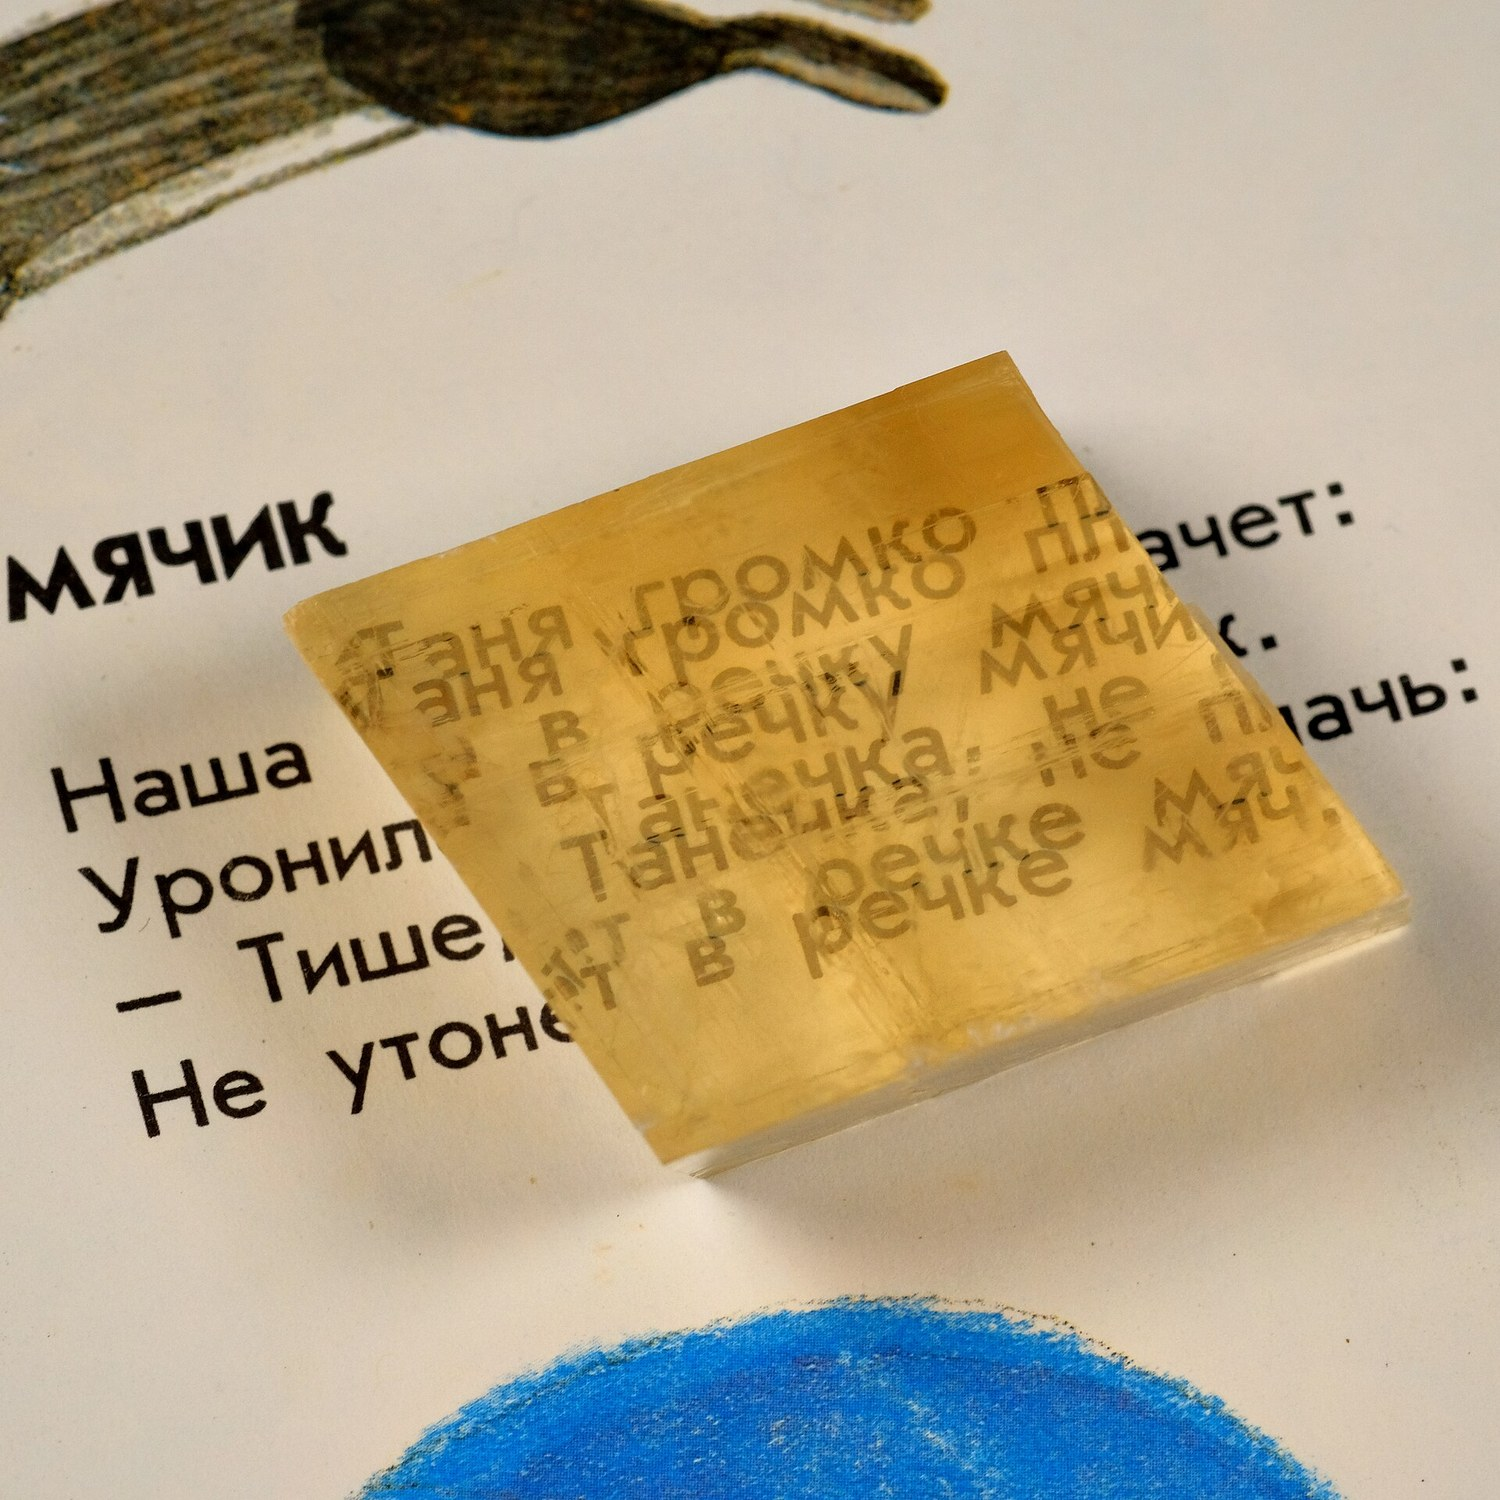
\includegraphics[width=0.72\textwidth]{../figures/an_calcite_birefringence.jpg}
\caption{一束光进晶体变成两束，因为两个偏振方向的折射率不同。等离子体在磁场里对光做的事与此同类，只是效应弱得多——本节的双折射公式，量级差距就在这张图里。}
\label{fig:photo-appan3}
\figsource{Masha Milshina，CC BY 4.0（Wikimedia Commons）}
\end{figure}

\section{科顿--穆顿效应：双折射里的三次方与一个单位陷阱}
\label{sec:app-an-cotton}

沿\textbf{垂直}磁场方向传播时，本征模换成两个线偏振：寻常模（$O$）与反常模（$X$）。
它们的折射率差在小 $Y$ 下展开为

\begin{equation}
\Delta n_{\mathrm{XO}}\equiv n_{\mathrm{X}}-n_{\mathrm{O}}
\simeq-\frac{XY^2}{2(1-X)^{3/2}}
\simeq-\frac12XY^2,
\label{eq:app-an-cotton}
\end{equation}

于是相位差（这一回\textbf{不做折半}，$X$ 与 $O$ 是线偏振，两支的相位差直接表现为椭圆率）

\begin{equation}
\varphi_{\mathrm{CM}}=\frac{\omega}{c}|\Delta n_{\mathrm{XO}}|L
=2.45682\times10^{-11}\,\lambda^3\!\!\int\! n_eB_\perp^2\,dl
\quad(\mathrm{rad}),
\label{eq:app-an-cmcoef}
\end{equation}

系数同样可以纯代数写出：$e^4/(16\pi^3c^4\varepsilon_0m_e^3)=2.45682\times10^{-11}$
（SI：$\lambda$ 用 m、$n_e$ 用 $\mathrm{m^{-3}}$、$B$ 用 T）。
\textbf{陷阱在这里}：文献里常见的写法是 $2.45\times10^{-19}$，配的是\textbf{高斯}。
因为 $1\ \mathrm{T}=10^4\ \mathrm{G}$，$B^2$ 差 $10^8$ 倍，
$2.45682\times10^{-11}$ 与 $2.45682\times10^{-19}$ 描述的是同一件事。
单位混用时会得到差一亿倍的所谓「异常」，而公式本身一个字都没错。

\begin{table}[htbp]
\centering
\caption{科顿--穆顿相位：垂直弦（$B_\perp=B_p=0.5\ \mathrm{T}$）与切向弦（$B_\perp\approx B_t$）的对比}
\label{tab:app-an-cotton}
\small
\begin{tabular}{p{3.2cm} p{2.8cm} p{3.0cm} p{4.4cm}}
\toprule
量 & 远红外 & CO$_2$ & 说明 \\
\midrule
$|\Delta n_{\mathrm{XO}}|$（垂直弦） & $1.29978\times10^{-8}$ & $8.22786\times10^{-13}$ & $\propto\lambda^3B_\perp^2$ \\
相位（精确解） & $0.15755^\circ$ & $0.000111775^\circ$ & 垂直弦，$B_\perp=0.5\ \mathrm{T}$ \\
相位（解析式） & $0.157345^\circ$ & $0.000111769^\circ$ & 与精确解差 $<0.2\%$ \\
$\varphi_{\mathrm{CM}}/\varphi_{\mathrm{FR}}$ & $0.000523241$ & $4.66864\times10^{-5}$ & 垂直弦上 CM 远小于 FR \\
切向弦放大 & $112.36$ 倍 & --- & $B_\perp^2$ 放大 $(B_t/B_p)^2$ \\
切向弦相位 & $17.6793^\circ$ & --- & 与 FR 同量级 \\
\bottomrule
\end{tabular}
\end{table}

表~\ref{tab:app-an-cotton} 说明了一件事：\textbf{科顿--穆顿的强弱取决于几何}。
垂直弦上 $B_\perp$ 只有极向场 $0.5\ \mathrm{T}$，相位小到 $0.15755^\circ$；
换成切向弦，$B_\perp$ 直接是环向场 $5.3\ \mathrm{T}$，相位跳到 $17.6793^\circ$（放大 $112.36$ 倍）。
这也是为什么偏振仪在设计阶段就要先画清楚「哪条弦看哪个分量」：
同一台机器上，FR 与 CM 对不同弦的敏感度可以差四个量级。

\begin{tip}{同一个 2.45，单位不同差一亿倍}{tip-app-an-cotton}
$2.45\times10^{-19}$ 里的 $B$ 是高斯，$2.45682\times10^{-11}$ 里的 $B$ 是特斯拉。
凡是遇到「某个效应大得离谱」的场合，先查公式约定的是哪套单位，
再查线积分里的 $B$ 是哪个分量，这两个坑占了这个领域一半的「异常」。
\end{tip}


\section{运动斯塔克效应：把投掷角读成安全因子剖面}
\label{sec:app-an-mse}

法拉第旋转给出的是 $\int n_eB_\parallel\,dl$，要拿到\textbf{局域}的磁场方向，
最主流的办法是往等离子体里打一束高能中性氢（或氘）原子，看它发的 $D_\alpha$ 线。
中性原子在磁场里运动时，在它的\textbf{静止系}里看到一个运动电场

\begin{equation}
\mathbf{E}_m=\mathbf{v}_b\times\mathbf{B},
\qquad
E_m=v_bB\sin\theta,
\label{eq:app-an-em}
\end{equation}

这个电场（不是实验室的电场）把 $n=3$ 能级按线性斯塔克效应劈开。

\begin{equation}
\Delta E=\frac{3}{2}\,n\,k\,e\,a_0E_m
\ \xrightarrow[\ n=3,\ |k|=2\ ]{}\ 9\,e\,a_0E_m
=1.25197\times10^{-21}\ \mathrm{J}=0.00781418\ \mathrm{eV},
\label{eq:app-an-stark}
\end{equation}

对应 $D_\alpha$（$656.28\ \mathrm{nm}$）的波长分裂。

\begin{equation}
\Delta\lambda=\frac{\lambda_0^2\Delta E}{hc}=2.71454\ \mathrm{nm},
\label{eq:app-an-split}
\end{equation}

而束内原子的热运动给出的多普勒宽度只有 $0.0677692\ \mathrm{nm}$，
分裂是它的 $40.0556$ 倍，所以两瓣干净地分开，不需要解卷积。
分裂的\textbf{方向}（各 $\pi$ 分量相对磁场的方位）由 $\mathbf{E}_m$ 定，
而 $\mathbf{E}_m\perp\mathbf{B}$，于是测量偏振方位就等于测量\textbf{磁场方向的投影}。

\begin{equation}
\tan\gamma=\frac{B_p}{B_t},
\qquad
q_{\mathrm{cyl}}=\frac{aB_t}{R_0B_p}
\ \xrightarrow[\ B_p/B_t=0.5/5.3\ ]{}\ \gamma=5.38931^\circ,\quad q_{\mathrm{cyl}}=3.41935 .
\label{eq:app-an-pitch}
\end{equation}

\begin{table}[htbp]
\centering
\caption{MSE 的工作点：$100\ \mathrm{keV}$ 氘束、$B_t=5.3\ \mathrm{T}$}
\label{tab:app-an-mse}
\small
\begin{tabular}{p{4.2cm} p{3.4cm} p{5.8cm}}
\toprule
量 & 数值 & 说明 \\
\midrule
束速度 $v_b$ & $3.09574\times10^{6}\ \mathrm{m\,s^{-1}}$ & $=0.0103263c$，能量 $100\ \mathrm{keV}$ \\
运动电场 $E_m$ & $16.4074\ \mathrm{MV\,m^{-1}}$ & $v_bB\sin\theta$，$\theta=90^\circ$ \\
最大斯塔克分裂 & $0.00781418\ \mathrm{eV}$ & $n=3$，$|k|=2$ \\
$D_\alpha$ 波长分裂 & $2.71454\ \mathrm{nm}$ & 观测量 \\
束内多普勒宽度 & $0.0677692\ \mathrm{nm}$ & $T_{\mathrm{beam}}=10\ \mathrm{eV}$ \\
分裂/多普勒 & $40.0556$ & 无需解卷积 \\
投掷角 $\gamma$ & $5.38931^\circ$ & $\arctan(B_p/B_t)$ \\
$\gamma$ 变 $1^\circ$ & $B_p$ 变 $18.6978\%$ & 诊断灵敏度 \\
\bottomrule
\end{tabular}
\end{table}

表~\ref{tab:app-an-mse} 最后两行说明 MSE 为何成为 $q$ 剖面的主力诊断，也暴露它的软肋：
$q$ 对投掷角的相对灵敏度是 $18.5005\%$ 每度（$1/\tan\gamma=10.6$ 每弧度）。
$1^\circ$ 的偏振定标误差就是 $18.5005\%$ 的 $q$ 误差。
MSE 的定标因此比它的光学部分更值钱。

\begin{tip}{MSE 测的是投掷角，不是磁场大小}{tip-app-an-mse}
分裂的\textbf{大小}正比于 $|\mathbf{E}_m|$，因此在束能量已知时也给出 $B$；
但真正被用起来的是分裂的\textbf{方位}，
它是磁场方向沿着束路径的投影，反演出来的就是安全因子 $q$ 的剖面。
把 MSE 当成「磁强计」会浪费它最值钱的那一半信息。
\end{tip}


\begin{figure}[htbp]
\centering
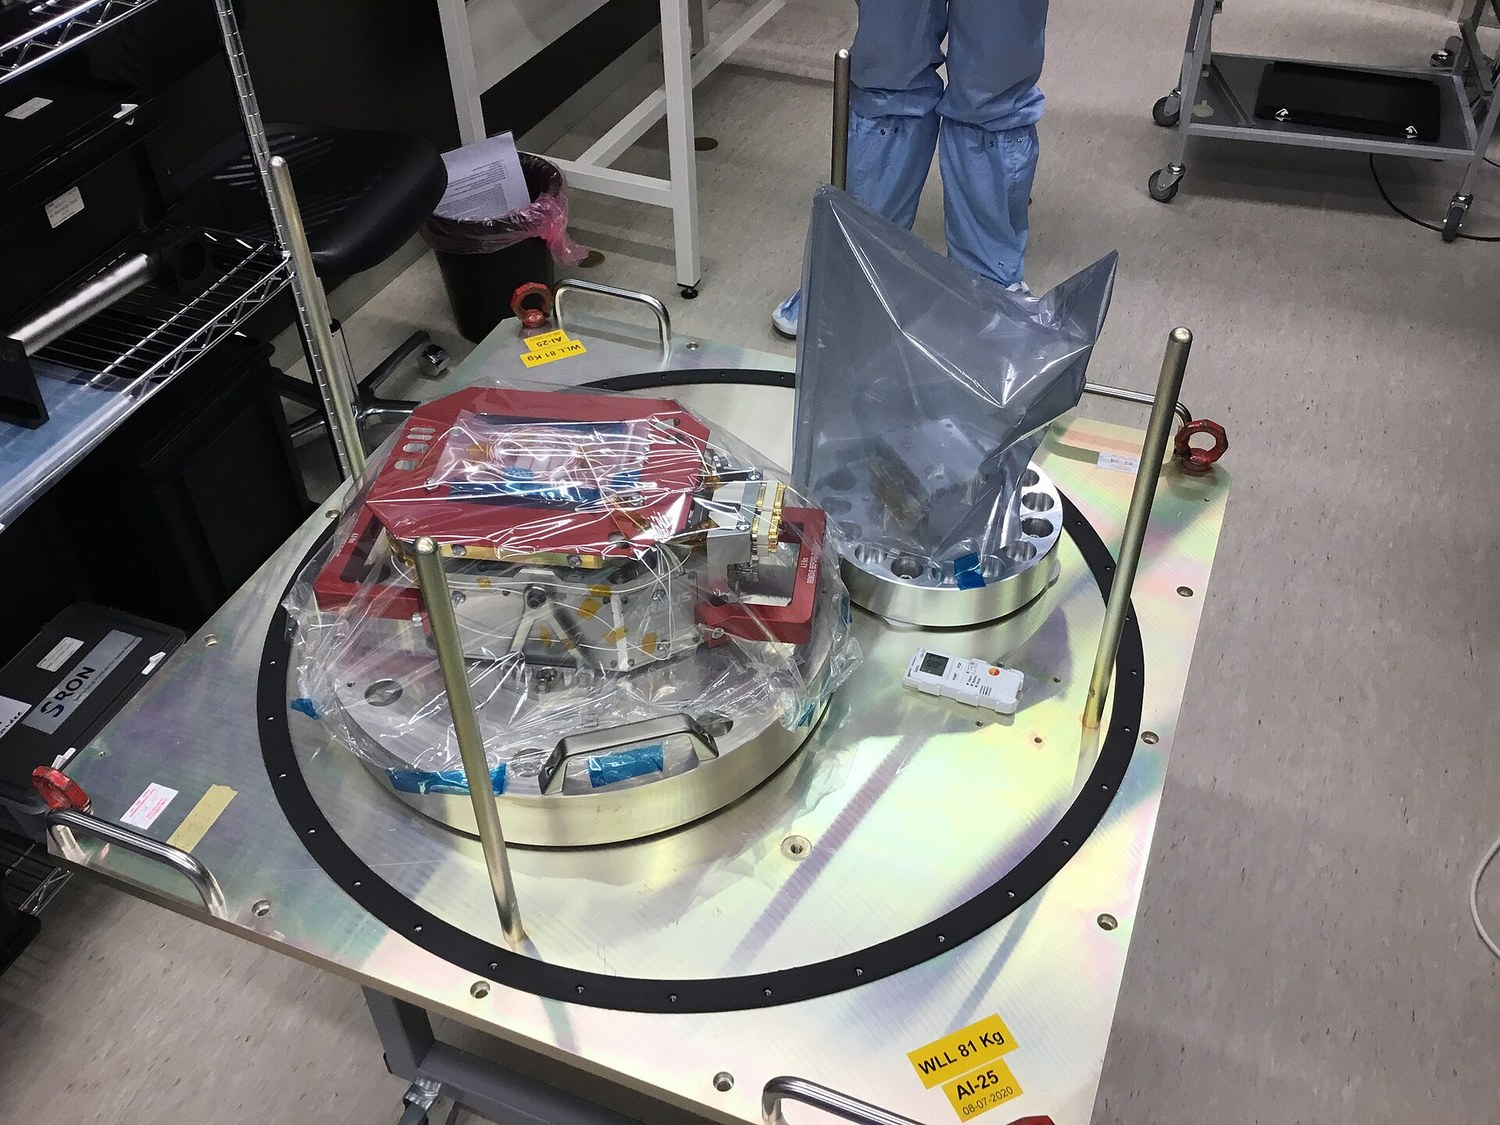
\includegraphics[width=0.72\textwidth]{../figures/spexone_polarimeter.jpg}
\caption{SPEXone 偏振仪：偏振是要被标定的物理量。偏振测量的难点不在「看见光」，而在把偏振态完整地解出来：调制、检偏与标定每一步都会引入系统误差。本节讲的相位—剖面反演与不确定度预算，与这类星载偏振仪用的是同一套语言。}
\label{fig:photo-appan2}
\figsource{NASA，Public domain（Wikimedia Commons）}
\end{figure}

\section{从相位到剖面：弦数、分辨率与不确定度}
\label{sec:app-an-inversion}

偏振仪和干涉仪一样，一根弦只给一个线积分。
要把线积分变成剖面，需要多根弦加一个反演模型（附录 Q 讲过 Abel 反演的基本形式）：

\begin{equation}
\varphi_i=\frac{2.63119\times10^{-13}}{2\pi}\lambda^2\!\!\int_{\text{弦 }i}\! n_eB_\parallel\,dl
\ \longrightarrow\
n_e(r),\,B_\parallel(r)\quad(\text{多弦联立}),
\label{eq:app-an-abel}
\end{equation}

反演的病态程度由\textbf{弦距}决定，而不是由相位分辨率决定。先算相位分辨率给出什么：

\begin{equation}
\delta\varphi=0.01^\circ=1.74533\times10^{-4}\ \mathrm{rad}
\ \Rightarrow\
\delta\!\int\! n_eB_\parallel dl=5.90355\times10^{18}\ \mathrm{T\,m^{-2}},
\label{eq:app-an-res}
\end{equation}

相对 $1.41333\times10^{21}\ \mathrm{T\,m^{-2}}$ 是 $0.417704\%$，
折算成等效平均磁场的分辨率是 $0.0221383\ \mathrm{T}$。
而几何给出的下限是：$9$ 根弦覆盖 $-a$ 到 $+a$，弦距 $0.5\ \mathrm{m}$；
中心弦的线积分是 $2.66667\times10^{20}\ \mathrm{m^{-2}}$，
边缘弦（$r=0.9a$）只有它的 $0.43589$ 倍。

\begin{table}[htbp]
\centering
\caption{分辨率账：相位分辨率、弦距与 $q$ 的灵敏度}
\label{tab:app-an-inversion}
\small
\begin{tabular}{p{4.4cm} p{3.2cm} p{5.8cm}}
\toprule
量 & 数值 & 说明 \\
\midrule
相位分辨率 & $0.01^\circ$ & 典型 PEM 偏振仪水平 \\
线积分分辨率 & $5.90355\times10^{18}\ \mathrm{T\,m^{-2}}$ & 相对 $0.417704\%$ \\
等效平均磁场分辨率 & $0.0221383\ \mathrm{T}$ & 单弦，$22.1383\ \mathrm{mT}$ \\
弦距（$9$ 弦） & $0.5\ \mathrm{m}$ & 空间分辨率上限 \\
边缘/中心线积分比 & $0.43589$ & $r=0.9a$ \\
$q$ 对 $\gamma$ 的灵敏度 & $18.5005\%$ 每度 & $1/\tan\gamma=10.6$ 每弧度 \\
$q=3$ 所需 $B_p$ & $0.569892\ \mathrm{T}$ & 当前值的 $1.13978$ 倍 \\
\bottomrule
\end{tabular}
\end{table}

表~\ref{tab:app-an-inversion} 给出一条实用判据：
当相位分辨率折算出的磁场分辨率（$0.0221383\ \mathrm{T}$）远小于弦距造成的空间模糊时，
\textbf{继续提高相位分辨率是浪费}；该做的是增加弦数或换几何。
这条判据与附录 Q 对探针阵列的说法相同。

\begin{tip}{线积分诊断的空间分辨率由弦距定，不由相位分辨率定}{tip-app-an-inversion}
$0.01^\circ$ 的相位分辨率已经是很好的水平，它折算出的磁场误差只有 $0.0221383\ \mathrm{T}$；
但 $9$ 根弦的弦距是 $0.5\ \mathrm{m}$，任何比这更细的结构都会被抹平。
诊断设计的第一步永远是数弦，而不是选探测器。
\end{tip}

\section{工程实现：调制、消光比与整圈模糊}
\label{sec:app-an-engineering}

偏振角不能直接「读」出来，只能把它调制起来再解调。
主流做法是\textbf{光弹调制器}（PEM）：一块被周期性挤压的石英，让两个正交方向的相位差按
$\sin(2\pi f_{\mathrm{PEM}}t)$ 振荡，于是偏振信号被搬到 $f_{\mathrm{PEM}}$ 及其谐波上。

\begin{equation}
S(t)\propto S_1\cos\delta(t)+S_2\sin\delta(t),
\qquad
\delta(t)=\delta_0\sin(2\pi f_{\mathrm{PEM}}t),
\qquad
f_{\mathrm{PEM}}=50\ \mathrm{kHz}\ \Rightarrow\ T_{\mathrm{PEM}}=20\ \mu\mathrm{s},
\label{eq:app-an-pem}
\end{equation}

在 $1\ \mathrm{ms}$ 内就有 $50$ 个调制周期，锁相解调后 $S_1$、$S_2$ 都拿到了，
偏振角 $\psi$ 与椭圆率 $\chi$ 也就同时拿到，
这正是 AN.3 节里 FR 与 CM 能在一台仪器上分离的原因。
\textbf{它们分别落在不同的解调通道里}。

\begin{equation}
\text{消光比 }10^{-3}\ \Rightarrow\ \delta\psi\approx\sqrt{10^{-3}}\ \mathrm{rad}=1.81185^\circ,
\label{eq:app-an-extinction}
\end{equation}

这个数字（$1.81185^\circ$）比相位分辨率（$0.01^\circ$）差了两个多量级，
说明\textbf{限制偏振仪精度的不是探测器，而是偏振元件的质量}。
沃拉斯顿棱镜、波片、窗片的应力双折射，都会以这个量级混进信号里。

第二个工程约束是 $2\pi$ 模糊。旋转角按 $\lambda^2$ 长，远红外波段一圈只有 $1.69198\times10^{21}\ \mathrm{T\,m^{-2}}$：

\begin{equation}
\varphi_{\mathrm{rot}}=2\pi
\iff
\int n_eB_\parallel\,dl=\frac{2\pi}{2.63119\times10^{-13}\lambda^2}
=1.69198\times10^{21}\ \mathrm{T\,m^{-2}},
\label{eq:app-an-ambiguity}
\end{equation}

而本工作点的线积分已经是 $1.41333\times10^{21}\ \mathrm{T\,m^{-2}}$，
即 $0.835315$ 圈，\textbf{再高一点密度就会翻过去}。
工程上的解法有三条：换短波长（CO$_2$ 只有 $2.39411^\circ$）、
用两个波长做粗定位、或者把弦分成几段各测一小段。
三条路都要付出代价（短波长丢 CM、分段丢弦数），
没有一条是纯赚的。

\begin{equation}
\text{定标：}\quad
B_\parallel^{\mathrm{cal}}=\frac{\varphi_{\mathrm{rot}}}{2.63119\times10^{-13}\lambda^2\!\int n_e\,dl},
\label{eq:app-an-calib}
\end{equation}

式~\eqref{eq:app-an-calib} 是 MSE 与偏振仪共用的定标式：
它要求\textbf{密度线积分}与\textbf{光路几何}都已知到优于目标精度一个量级，
否则误差会原封不动地搬到磁场头上（AN.2 节说过的那条纪律）。

\begin{table}[htbp]
\centering
\caption{工程约束一览：调制、消光比、模糊与定标}
\label{tab:app-an-engineering}
\small
\begin{tabular}{p{4.4cm} p{3.4cm} p{5.6cm}}
\toprule
量 & 数值 & 说明 \\
\midrule
PEM 频率 & $50\ \mathrm{kHz}$ & 周期 $20\ \mu\mathrm{s}$ \\
$1\ \mathrm{ms}$ 内周期数 & $50$ & 锁相带宽足够 \\
消光比 $10^{-3}$ 的相位误差 & $1.81185^\circ$ & 元件质量是主要限制 \\
FR 的 $2\pi$ 对应线积分 & $1.69198\times10^{21}\ \mathrm{T\,m^{-2}}$ & 远红外 \\
工作点占一圈的比例 & $0.835315$ & 已接近模糊 \\
CO$_2$ 的旋转角 & $2.39411^\circ$ & 无模糊 \\
切向弦 CM 相位 & $17.6793^\circ$ & 与 FR 同量级 \\
\bottomrule
\end{tabular}
\end{table}

\begin{tip}{整圈模糊不是噪声，是设计约束}{tip-app-an-engineering}
噪声可以让多次测量平均掉，模糊不能，它把「$0.835315$ 圈」和「$1.835315$ 圈」变成同一个读数。
凡是按 $\lambda^2$ 或 $\lambda^3$ 标度的诊断量，选波长时都要先问一句：
\textbf{最坏情况下会不会超过一圈}？
超过的话，方案要么改，要么补一条独立的粗测量通道。
\end{tip}


\section{估算练习}
\label{sec:app-an-problems}

\begin{enumerate}
\item \textbf{练习 1}（波长选择）把远红外激光（$118.8\ \mu\mathrm{m}$）换成 CO$_2$（$10.6\ \mu\mathrm{m}$），
旋转角变成原来的几分之一？在本工作点上远红外的旋转角是几圈？
\item \textbf{练习 2}（密度减半）若芯部密度降到 $0.5\times10^{20}\ \mathrm{m^{-3}}$（剖面形状不变），
$\int n_eB_\parallel\,dl$ 与 CO$_2$ 的旋转角各是多少？
\item \textbf{练习 3}（极向场加倍）若 $B_p$ 变成 $1.0\ \mathrm{T}$，垂直弦上的科顿--穆顿相位变成多少？为什么是四倍而不是两倍？
\item \textbf{练习 4}（束能提高）束能提到 $150\ \mathrm{keV}$，束速度、运动电场、$D_\alpha$ 分裂各是多少？
相对 $100\ \mathrm{keV}$ 大了几倍？
\item \textbf{练习 5}（弦数）把弦数从 $9$ 增到 $13$，弦距与相邻弦的线积分差各是多少？
\item \textbf{练习 6}（分辨率）若相位分辨率做到 $0.005^\circ$，线积分分辨率与相对精度各是多少？
\end{enumerate}

\textbf{解答}

\textbf{解答 1}
旋转角按 $\lambda^2$ 标度，所以
$(118.8/10.6)^2=125.609$ 倍（远红外更大）。
远红外的旋转角是 $5.24844\ \mathrm{rad}=300.713^\circ=0.835315$ 圈；
CO$_2$ 只有 $2.39404^\circ$，因此 CO$_2$ 没有 $2\pi$ 模糊，代价是科顿--穆顿小到可以忽略。

\textbf{解答 2}
$\int n_eB_\parallel\,dl$ 减半为 $7.06667\times10^{20}\ \mathrm{T\,m^{-2}}$，
CO$_2$ 的旋转角减半为 $1.19702^\circ$。

\textbf{解答 3}
科顿--穆顿相位正比于 $B_\perp^2$，$B_p$ 加倍使相位变 $4$ 倍，
即 $0.157345^\circ\rightarrow0.629382^\circ$。
它不是两倍，因为电场对介质的作用本身还带一个因子 $B$（式~\eqref{eq:app-an-cotton}）。

\textbf{解答 4}
$v_b=\sqrt{2E/m_D}=3.79149\times10^{6}\ \mathrm{m\,s^{-1}}$，
$E_m=v_bB_t=20.0949\ \mathrm{MV\,m^{-1}}$，
$\Delta\lambda=3.32461\ \mathrm{nm}$，
相对 $100\ \mathrm{keV}$ 都大 $\sqrt{1.5}=1.22474$ 倍，
因为速度按 $\sqrt{E}$ 长，而斯塔克分裂又正比于速度。

\textbf{解答 5}
弦距 $=2a/12=0.333333\ \mathrm{m}$；
相邻弦的线积分差 $=1.10336\times10^{19}\ \mathrm{m^{-2}}$
（中心附近差最小，边缘最大，这里给的是边缘相邻弦的差值口径）。

\textbf{解答 6}
线积分分辨率 $=2.95177\times10^{18}\ \mathrm{T\,m^{-2}}$，
相对 $1.41333\times10^{21}\ \mathrm{T\,m^{-2}}$ 是 $0.208852\%$。
按 AN.5 节的判据，这个精度已经远超弦距造成的空间模糊，
\textbf{再往下压相位分辨率没有收益}。

\section{来源、分级与版权说明}

\begingroup\small
本附录的数字都可以用 \texttt{tools/\allowbreak{}calc/\allowbreak{}appAN\_calc.py} 重算一遍；脚本与当时的输出记录都在仓库里。
\label{sec:app-an-source}

\subsection*{本附录的借鉴来源}

\begin{table}[htbp]
\centering
\caption{本附录的借鉴来源与处理方式}
\label{tab:app-an-source}
\small
\begin{tabular}{p{3.6cm} p{4.6cm} p{5.4cm}}
\toprule
借鉴内容 & 来源 & 本书的处理 \\
\midrule
偏振诊断总框架、Stokes 参数与仪器口径 & Hutchinson《Principles of Plasma Diagnostics》2nd ed. 2002 第 6 章 & 重写推导，只保留结论与可复算的系数 \\
偏振诊断在托卡马克中的位置（FR、CM、MSE） & Wesson《Tokamaks》4th ed. 2011 第 12 章 & 改写为「先算量级、再谈方案」的叙述 \\
线性斯塔克效应与谱线分裂 & Griem《Principles of Plasma Spectroscopy》1997；Fujimoto《Plasma Spectroscopy》2004 & 只用能级分裂公式与量级 \\
谱线测量与仪器展宽 & Kunze《Introduction to Plasma Spectroscopy》2009 & 与附录 AH 的口径对齐 \\
MSE 原理与首次实现 & Levinton 等, Phys. Rev. Lett. 63, 2060 (1989) & 只引用其原理结论，不复制装置细节 \\
MSE 数据分析与定标 & Wróblewski 与 Lao, Rev. Sci. Instrum. 63, 5140 (1992) & 只引用定标思路 \\
原子物理与谱线展宽 & Salzmann《Atomic Physics in Hot Plasmas》1998 & 与附录 AH 同源，不重复 \\
\bottomrule
\end{tabular}
\end{table}

\subsection*{不复制什么}

\begin{itemize}
\item 不复制文献中偏振仪的光路图、探测器布置与机械结构细节；
\item 不复制各文献使用的符号体系（本书统一用 $X$、$Y$、$\varphi_{\mathrm{rot}}$、$\varphi_{\mathrm{CM}}$）；
\item 不复制原始论文中对 MSE 定标流程的逐步操作描述；
\item 不复制任何教科书或论文中的习题原题。
\end{itemize}

\begin{tip}{本附录没有涵盖什么}{tip-app-an-honest}
这一篇不展开偏振仪的工程设计、锁相解调的电路细节、
也不给真实装置上的误差预算表。
它只把「偏振怎么变成磁场与 $q$」这条链条上的每一步量级算清楚，其余的留给专门文献。
\end{tip}
\endgroup
